\documentclass{article}
\usepackage{graphicx}
\usepackage{geometry}
\usepackage{hyperref}
\usepackage{amsmath}
\usepackage{amssymb}
\geometry{a4paper, margin=1in}

\title{High-Level Design Document for Vacume robot }
\author{Arel Sharon 323012971 and 
Matan Amichai 315441972}
\date{\today}

\begin{document}

\maketitle

\tableofcontents

\newpage

\section{Introduction}
This document provides the high-level design (HLD) for the EX02 robot Cleaning project. It includes the UML class diagram, UML sequence diagram, design considerations, alternatives, and the testing approach used in the project.

\section{UML Class Diagram}
The following class diagram represents the key classes and their relationships in the upgraded House Cleaning project.

\begin{figure}[h!]
    \centering
    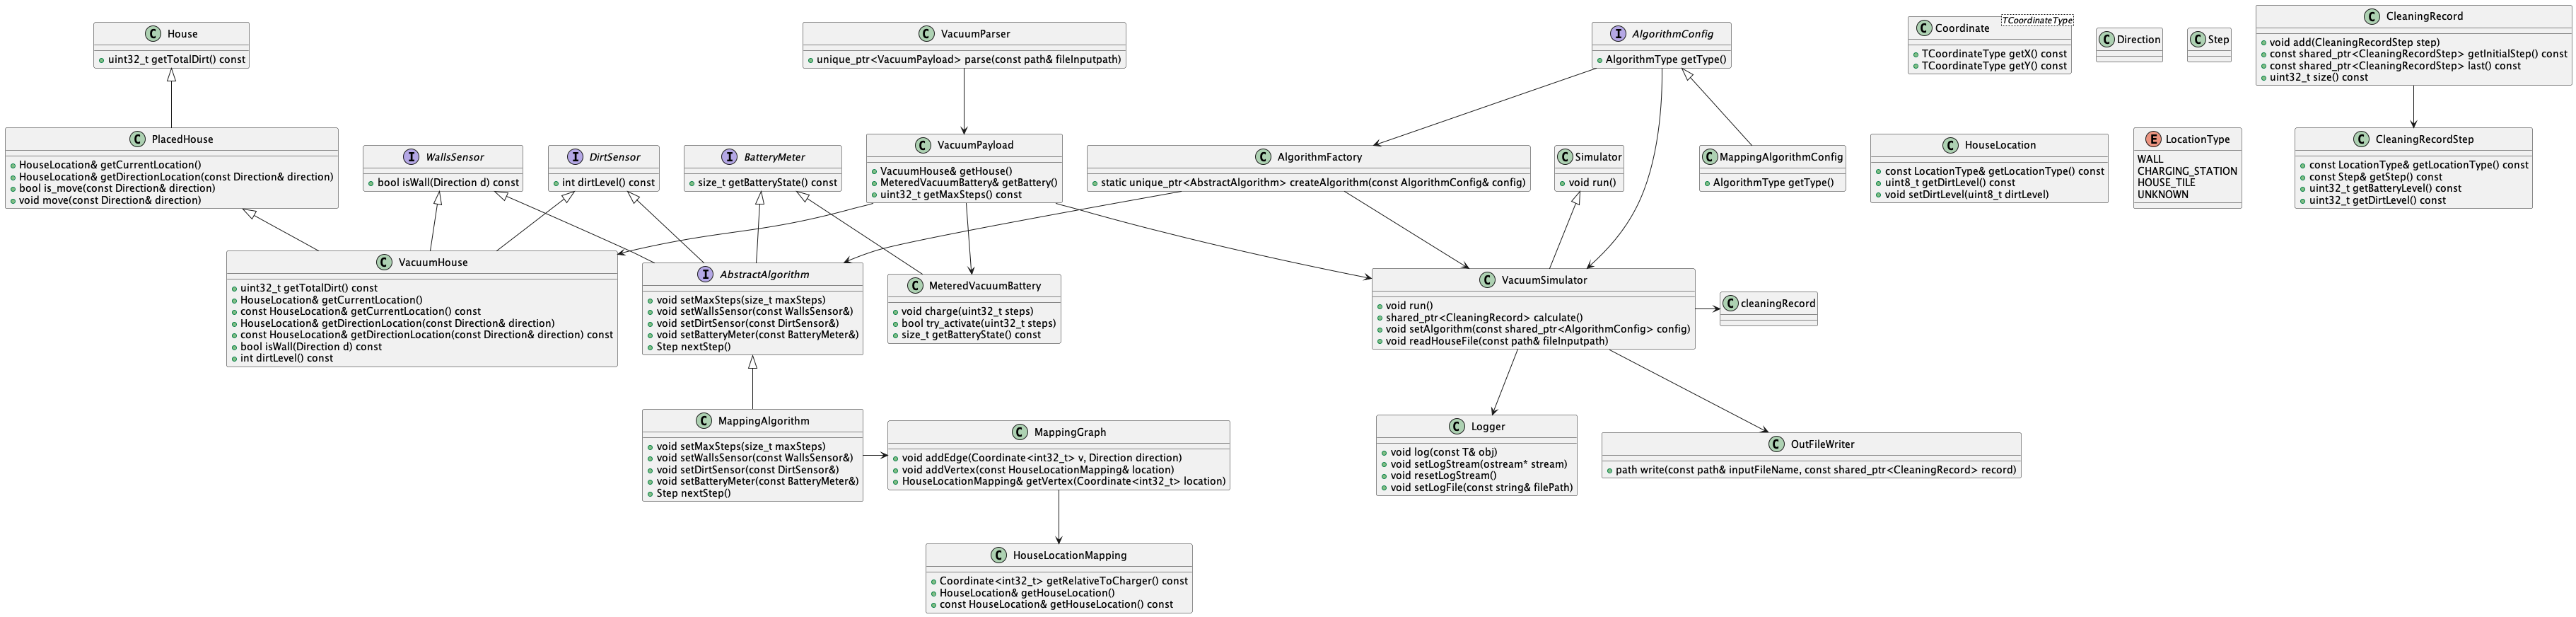
\includegraphics[width=\textwidth,height=0.5\textheight,keepaspectratio]{Diagrams/output_directory/class_diagram.png}
    \caption{UML Class Diagram}
    \label{fig:class-diagram}
\end{figure}

\section{UML Sequence Diagram}
The sequence diagram below illustrates the main flow of the upgraded House Cleaning, including the interaction between different classes during the cleaning process.

\begin{figure}[h!]
    \centering
    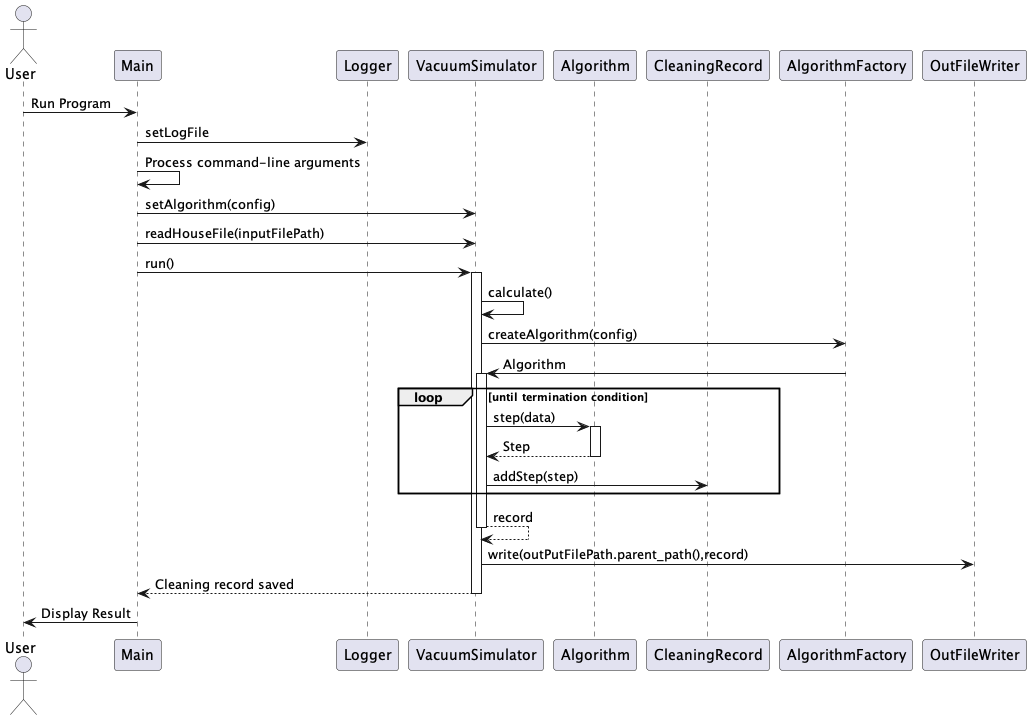
\includegraphics[width=\textwidth]{Diagrams/output_directory/sequence_diagram.png}
    \caption{UML Sequence Diagram}
    \label{fig:sequence-diagram}
\end{figure}

\section{Design Considerations and Alternatives}
\subsection{Design Considerations}
\begin{itemize}
    \item \textbf{MappingGraph}
        \begin{itemize}
            \item The algorithm maintains a graph represented by a variation on adjacency list
            \item The graph maps vertexes internally using an incrementing int id but exposes an API that allows the user to refer to vertexes as their relative location to the charger which is what the algorithm is aware of. This allows the user to easily query locations in the graph while the graph can use the lightweight representation of vertex's for expensive operations such as bfs.
            \item The graph exposes a Bfs Find First function similar to the find first of function provided by std, this function receives a starting location and condition(as predicate) and steps BFS until the condition is met. This improves performance as most of our operations are of the "first first location to be something" type, such as find the closest path to charger(so first location to have a charging station mapping), find closest dirt etc.
        \end{itemize}
        \item  \textbf{Parsing}
            \begin{itemize}
                \item File parsing
                    \begin{itemize}
                        \item Reads the input file and extracts parameters such as max steps and max battery steps using a simple regex to handle any white space problems.
                        \item Verify that the inputs are valid 
                        \item In the case of any error E.g file not found/ improperly structured, bad values etc terminate.
                    \end{itemize}
                \item Component parsing: 
                    \begin{itemize}
                        \item Constructs components like VacuumBattery and VacuumHouse from the parsed data.
                        \item  Note that we know that the simple input parameters are correct but have no idea if the broader house structure is valid. This decision is left to the House Constructor as it may differ house by house.
                   \end{itemize}
       \end{itemize}
        Unless error are found in construction we return a uniqueptr to our run payload(a wrapper around the parsed components) This is a unique pointer because it should only be held by the simulator as the objects inside are mutable. Also, we dont want to copy the Payload object as it can be quite large.
        
    \item \textbf {Sensors} We noticed early on that we had already implemented the functions that are described by the Sensors provided. That led us to tread the sensor as "Interfaces" which we implemented in both our main stateful classes
    \begin{itemize}
        \item VacuumHouse That is responsible for maintaining the position of the vacuum in the house, movement and dirt positions and amounts. The class exposes an API to simulator that is limited to moves that are possible under restrictions. E.g Simulator cannot in error move the vacuum 2 steps in a single turn (Singular step required by house API) neither can he move into a wall (moving into a wall will result in error message and no move made).
        \item MeteredVacuumBattery Is responsible for charging,discharging,over charging, etc this allows us to hide things like charging formula, max and min battery checks and  compensation for round down error due to inherent double inaccuracy under a single API
    \end{itemize}

    This allows us to set the sensors at the beginning of the run and completely forget about them, as they report their value based on the state of the run which is already updated.
    \item \textbf {Output Generation} Neither the algorithm nor the simulator write directly to output files. An external class is used by the simulator that translate a record of actions taken by the algorithm to an output file, allowing for multiple output formats for a single run.
    \item \textbf{Error Handling}:
    \begin{itemize}
         \item Utilizes std::optional and runtime exceptions for error communication.
         \item Internal functions use optionals for error handling, while components throw detailed exceptions.
         \item Parsing errors result in null optionals, leading to informative error messages.
         \item Invalid algorithm steps result in a null optional, stopping the vacuum and returning completed steps.
         \item All errors are logged for debugging and error tracking.
    \end{itemize}
\end{itemize}

\subsection{Design Alternatives}
\begin{itemize}
    \item We opted for a more general graph approach(or at least an approach that *could* be easily generalised) this was mainly to make sure that implementing graph algorithms is relatively easy. Creating a specialised graph implementation for the specific mapping scenario could have allowed us to utilise some of the unique cases that are present in the project such as every vertex having at most 4 edges(For each direction), etc  to optimize our approach at the cost of maybe complicating the implementation of future algorithms.
\end{itemize}

\section{Testing Approach}
The testing strategy for the upgraded House Cleaning project involves unit tests and end-to-end tests using the Google Test framework and a bash script.

\section{Unit Tests}
Unit tests ensure the isolated functionality of individual classes and methods using GTest. Classes with corresponding unit tests include:

\subsection{CleaningRecord}
\begin{itemize}
    \item \textbf{Tests}:
    \begin{itemize}
        \item \textbf{Construction}: Ensures proper construction and initialization.
        \item \textbf{Add}: Validates step addition and size incrementation.
        \item \textbf{InitialValue}: Verifies initial values and the behavior of \texttt{getInitialStep}.
    \end{itemize}
\end{itemize}

\subsection{HouseLocation}
\begin{itemize}
    \item \textbf{Tests}:
    \begin{itemize}
        \item \textbf{Construction}: Checks various location types and initial dirt levels.
        \item \textbf{SetDirtLevel}: Ensures dirt level setting within allowed limits and throws exceptions for invalid values.
        \item \textbf{GetDirtLevel}: Validates the retrieval of the current dirt level.
    \end{itemize}
\end{itemize}

\subsection{MappingAlgorithm}
\begin{itemize}
    \item \textbf{Tests}:
    \begin{itemize}
        \item \textbf{FutileTest}: Ensures the algorithm handles minimal and locked-in houses correctly.
        \item \textbf{MappingTest}: Validates mapping in various house configurations, including lines and big empty spaces.
        \item \textbf{CleaningTest}: Checks the cleaning process in different house layouts and battery levels.
    \end{itemize}
\end{itemize}

\subsection{MeteredVacuumBattery}
\begin{itemize}
    \item \textbf{Tests}:
    \begin{itemize}
        \item \textbf{ActivateCorrectly}: Validates battery activation and decrements correctly.
        \item \textbf{ActivateOvercharge}: Ensures activation does not exceed the battery limit.
        \item \textbf{Charge}: Checks the charging functionality.
        \item \textbf{TrickleCharge}: Verifies slow charging behavior.
        \item \textbf{OverCharge}: Ensures battery does not overcharge.
    \end{itemize}
\end{itemize}

\subsection{OutFileWriter}
\begin{itemize}
    \item \textbf{Tests}:
    \begin{itemize}
        \item \textbf{WORKING}: Validates the correct output file format for a working state.
        \item \textbf{DEAD}: Ensures proper file output for a dead vacuum state.
        \item \textbf{WithoutStep}: Checks file output when no steps are recorded.
        \item \textbf{FINISHED}: Validates file output for a finished cleaning process.
        \item \textbf{HandleNoRecord}: Ensures no output file is created when no record exists.
        \item \textbf{CreateDirectoryIfNotExists}: Validates directory creation if it does not exist.
    \end{itemize}
\end{itemize}

\subsection{VacuumHouse}
\begin{itemize}
    \item \textbf{Tests}:
    \begin{itemize}
        \item \textbf{Construction}: Ensures proper construction and handling of invalid configurations.
        \item \textbf{getAtPosition}: Validates the retrieval of locations at specific positions.
        \item \textbf{move}: Checks the movement functionality within the house.
        \item \textbf{isMove}: Ensures movement validation in all directions.
        \item \textbf{outOfBoundsDirtCount}: Checks the total dirt count for out-of-bounds scenarios.
    \end{itemize}
\end{itemize}

\subsection{VacuumParser}
\begin{itemize}
    \item \textbf{Tests}:
    \begin{itemize}
        \item \textbf{ParseInvalidHouses}: Ensures the parser handles invalid house configurations correctly.
        \item \textbf{ParseValidHouses}: Validates the parser for various valid house configurations.
        \item \textbf{CheckParsing}: Checks the accuracy of parsed house details.
    \end{itemize}
\end{itemize}


\subsection{End-to-End Tests}
End-to-end tests use a bash script to compile and run the application.
\begin{itemize}
    \item Unit tests for MappingAlgorithmTest generate output files in the `/test/example/gt` directory. The script runs these inputs and compares results to expected outputs.
    \item Fail tests in the `/test/failtests` directory ensure invalid inputs are correctly handled.
    \item The script verifies program behavior with incorrect arguments and optional parameters.
    \item Valgrind is used to detect and alert potential memory leaks during testing.
\end{itemize}

\subsection{Additional Testing Options}
\begin{itemize}
    \item The `/test/examples` directory contains input files for manual testing of the application.
\end{itemize}

\end{document}
